%
% Chapter 10
%

\chapter{STATISTICAL METHODS AND RESULTS}
\label{chap:stats}
The \tth signal process, as well as the backgrounds, are inherently subject to randomness due to quantum mechanics.
Additional statistical fluctuations are introduced in the measurement process. This inherent randomness means that simply counting the number of predicted
signal and background events, and counting the number of events observed from data and comparing the two numbers is not necessarily enough to infer the presence or
lack thereof of the \tth signal process. Instead, the degree to which the
number of events in the signal and background predictions agree, given their uncertainties, with the number of events observed in data, must be quantified.
Furthermore we must quantify the probability that, and the extent to which, the numbers we observe are not due to statistical fluctuations driven by randomness. 
To quantitatively estimate how well the prediction, the existence of the SM \tth signal and corresponding backgrounds, agree with the observation in data,
we use techniques based on the likelihood function.
%We use the likelihood function as the basis for estimating the signal strength parameter via the maximum likelihood technique, and also for composing our test statistic when
%calculating upper limits  on the signal strength parameter via the CLs method. 

\section{Maximum Likelihood Fit, Signal Strength}
\label{sec:fit}
The primary purpose of this analysis is to determine the extent to which there exists a SM \tth signal in the observed data. This is quantified with the signal strength
parameter $\mu$, which is determined from the Maximum Likelihood Estimator (MLE) method. 
The likelihood function is defined as the probability density of the number of observed events, $N$, given the predicted number of signal-plus-background events, $\mu$s$ + b$,
where $\mu$ is the signal strength parameter we wish to estimate.
The signal strength parameter is a modifier (multiplier) on the SM cross section of the \tth signal process, defined as $\mu = \sigma(\tth)/\sigma_{SM}(\tth)$.
The signal strength parameter $\mu$ is more generally referred to as the parameter of interest (POI), and it is free to float to the value which best fits the observation.
The simplified likelihood, ignoring nuisance parameters for now, is written as a Poisson probability as:

\begin{equation}
\label{eqn:likelihood1}
\mathcal{L}(data|\mu) = P(N|\mu s+b) = \frac{(\mu s+b)^{N}e^{-(\mu s+b)}}{N!}
\end{equation}

\noindent The above expression holds for a single bin of events; however, this analysis is performed in each subcategory of the signal
region for each bin of the final BDT discriminant.
As each bin in each subcategory is statistically independent, the overall likelihood for this analysis is then the product of the
separate likelihoods for each bin in each subcategory, $i$,
calculated given the cooresponding predictions of signal and background yields $s_{i}, b_{i}$ and number of events observed in data $n_{i}$ as:

\begin{equation}
\label{eqn:likelihood2}
\mathcal{L}(data|\mu) = \prod_{i=1} \frac{(\mu s_{i}+b_{i})^{n_{i}}e^{-(\mu s_{i}+b_{i})}}{n_{i}!}
\end{equation}

\noindent Now the uncertainties associated with the signal and background predictions must be accounted for in the form of nuisance parameters. The expected signal
and background yields are re-written $s \rightarrow s(\theta)$ and $b \rightarrow b(\theta)$ to depend on the set of nuisance parameters $\theta$.
The expected value of the nuisance parameters is $\tilde{\theta}$.
We now calculate the probability that we would have previously measured the nuisance parameters and obtained the expected value $\tilde{\theta}$, given that the
true value is $\theta$: $\rho(\tilde{\theta}|\theta)$. In this analysis, $\rho$ is a gaussian distribution for shape systematics,
and a log-normal distribution for rate systematics.

\begin{equation}
\label{eqn:likelihood3}
\mathcal{L}(data|\mu,\theta) = \prod_{i=1} \frac{(\mu s_{i}(\theta)+b_{i}(\theta))^{n_{i}}e^{-(\mu s_{i}(\theta)+b_{i}(\theta))}}{n_{i}!} \cdot \rho(\tilde{\theta}|\theta)
\end{equation}

\noindent The estimated value for $\mu$ is obtained from finding the values of $\mu$ and $\theta$ which maximize the likelihood, denoted as $\hat{\mu}$ and $\hat{\theta}$.
This frequentist technique is called the maximum likelihood estimation (MLE)~\cite{lista} and the general technique of measuring nuisance parameter values based on a fit
to data is called ``profiling''.
In practice, we first take the negative log of the likelihood (NLL), and then find the minimum, since it simplifies
the procedure by turning the product in Equation~\ref{eqn:likelihood3} into a sum. $\hat{\mu}$ is referred to as the ``best-fit'' $\mu$, because it is the value which best fits the data.
This maximum likelihood procedure is also referred to generally as the ``fit''~\cite{CMS-AN-11-298}. 

This signal strength $\mu$ is the factor by which the expected \tth yields are multiplied, without altering the branching fractions, to best-fit the observation in data
while the backgrounds are constrained to SM predictions within their systematic uncertainties.
The observed  best fit signal strength for the SM \tth hypothesis is 1.7$^{+0.6}_{-0.5}$ times the SM expectation,
corresponding to an observed significance of 3.3$\sigma$, as shown in Table~\ref{tab:mu}.
This observation should be compared to the expected best fit signal strength for the SM \tth hypothesis is 1.0$^{+0.5}_{-0.5}$ times the SM expectation,
corresponding to an expected significance of 2.1$\sigma$, as shown in Table~\ref{tab:mu}.
The observed signal strength and significance result from comparing the observed data to the signal and background predictions from the SM with the MLE,
while the expected signal strength and significance are obtained the same way, but replacing the observed data with the SM predictions for signal and background.
The post-fit yields for the expected signal and background processes are listed by lepton flavor in Table~\ref{tab:postfit_yields}.
The impacts of the statistical, theoretical, and experimental sources of uncertainty, as well as the post-fit values of the nuisances and their correlation with
the fitted signal strength is shown in Figure~\ref{fig:impacts}. The impact of a nuisance parameter on the POI, $\mu$, is defined as the shift
from varying $\theta$ to its $+1\sigma$ or $-1\sigma$ post-fit values ($\pm\Delta\theta$) with all other nuisances fixed to their post-fit values:
$\pm\Delta\mu = \hat{\mu}(\hat{\theta}\pm\Delta\theta) -\hat{\mu}(\hat{\theta})$. The impacts help illustrate which nuisance parameters have the largest effect on
the POI uncertainty. 


\begin{table}[htbp]
\begin{center}
  \caption[Table of best-fit signal strength]{}
    \begin{tabular}{c c c} \hline
      Observed $\mu$ fit $\pm$1$\sigma$ & Expected $\mu$ fit $\pm$1$\sigma$ & Observed(expected) significance & \\ \hline 
      1.7$^{+0.6}_{-0.5}$ & 1.0$^{+0.5}_{-0.5}$ & 3.3$\sigma$ (2.1$\sigma$)  \\
      \hline
    \end{tabular}
    \label{tab:mu}
\end{center}
\end{table}


\begin{table}[htbp]
  \begin{center}
    \caption[Signal region post-fit event yields by lepton flavor]{Expected post-fit yields 
      for signal and background predictions, and observed yields in data. Yields
      are shown after a fit to data with all predictions constrained to SM expectation.
      The (post-fit) uncertainties shown are from profiling the nuisance parameters to best-fit the data.}
    \begin{tabular}{l c c c} \hline
      & $\mu\mu$ & $ee$ & $e\mu$  \\ \hline 
      $t\bar{t}W$ & 51.2 $\pm$ 2.6 & 20.4 $\pm$ 1.0 & 72.9 $\pm$ 3.4 \\
      $t\bar{t}Z/\gamma^{*}$ & 17.9 $\pm$ 0.9 & 16.0 $\pm$ 1.0 & 44.9 $\pm$ 2.0 \\
      \hline
      WZ & 6.8 $\pm$ 2.6 & 2.0 $\pm$ 0.8 & 10.0 $\pm$ 3.5 \\
      Rare SM. bkg & 7.2 $\pm$ 0.8 & 4.0 $\pm$ 0.4 & 12.5 $\pm$ 1.1 \\
      WWss & 3.6 $\pm$ 0.7 & 1.8 $\pm$ 0.3 & 5.5 $\pm$ 1.0 \\
      \hline
      Conversions & 0.0 $\pm$ 0.0 & 10.7 $\pm$ 6.3 & 7.4 $\pm$ 1.2 \\
      Charge flip & 0.0 $\pm$ 0.0 & 9.2 $\pm$ 0.8 & 14.2 $\pm$ 1.2 \\
      Non-prompt leptons & 31.9 $\pm$ 5.8 & 18.4 $\pm$ 2.4 & 56.7 $\pm$ 7.3 \\
      \hline
      Total bkg & 118.6 $\pm$ 7.0 & 82.6 $\pm$ 7.0 & 224.1 $\pm$ 9.3 \\
      \hline
      $t\bar{t}H$ & 19.5 $\pm$ 1.4 & 7.9 $\pm$ 0.6 & 27.6 $\pm$ 1.9 \\
      \hline
      Data & 154 & 95 & 274 \\
      \hline
    \end{tabular}
    \label{tab:postfit_yields}
  \end{center}
\end{table}

\begin{figure}[htb]
        \centering 
        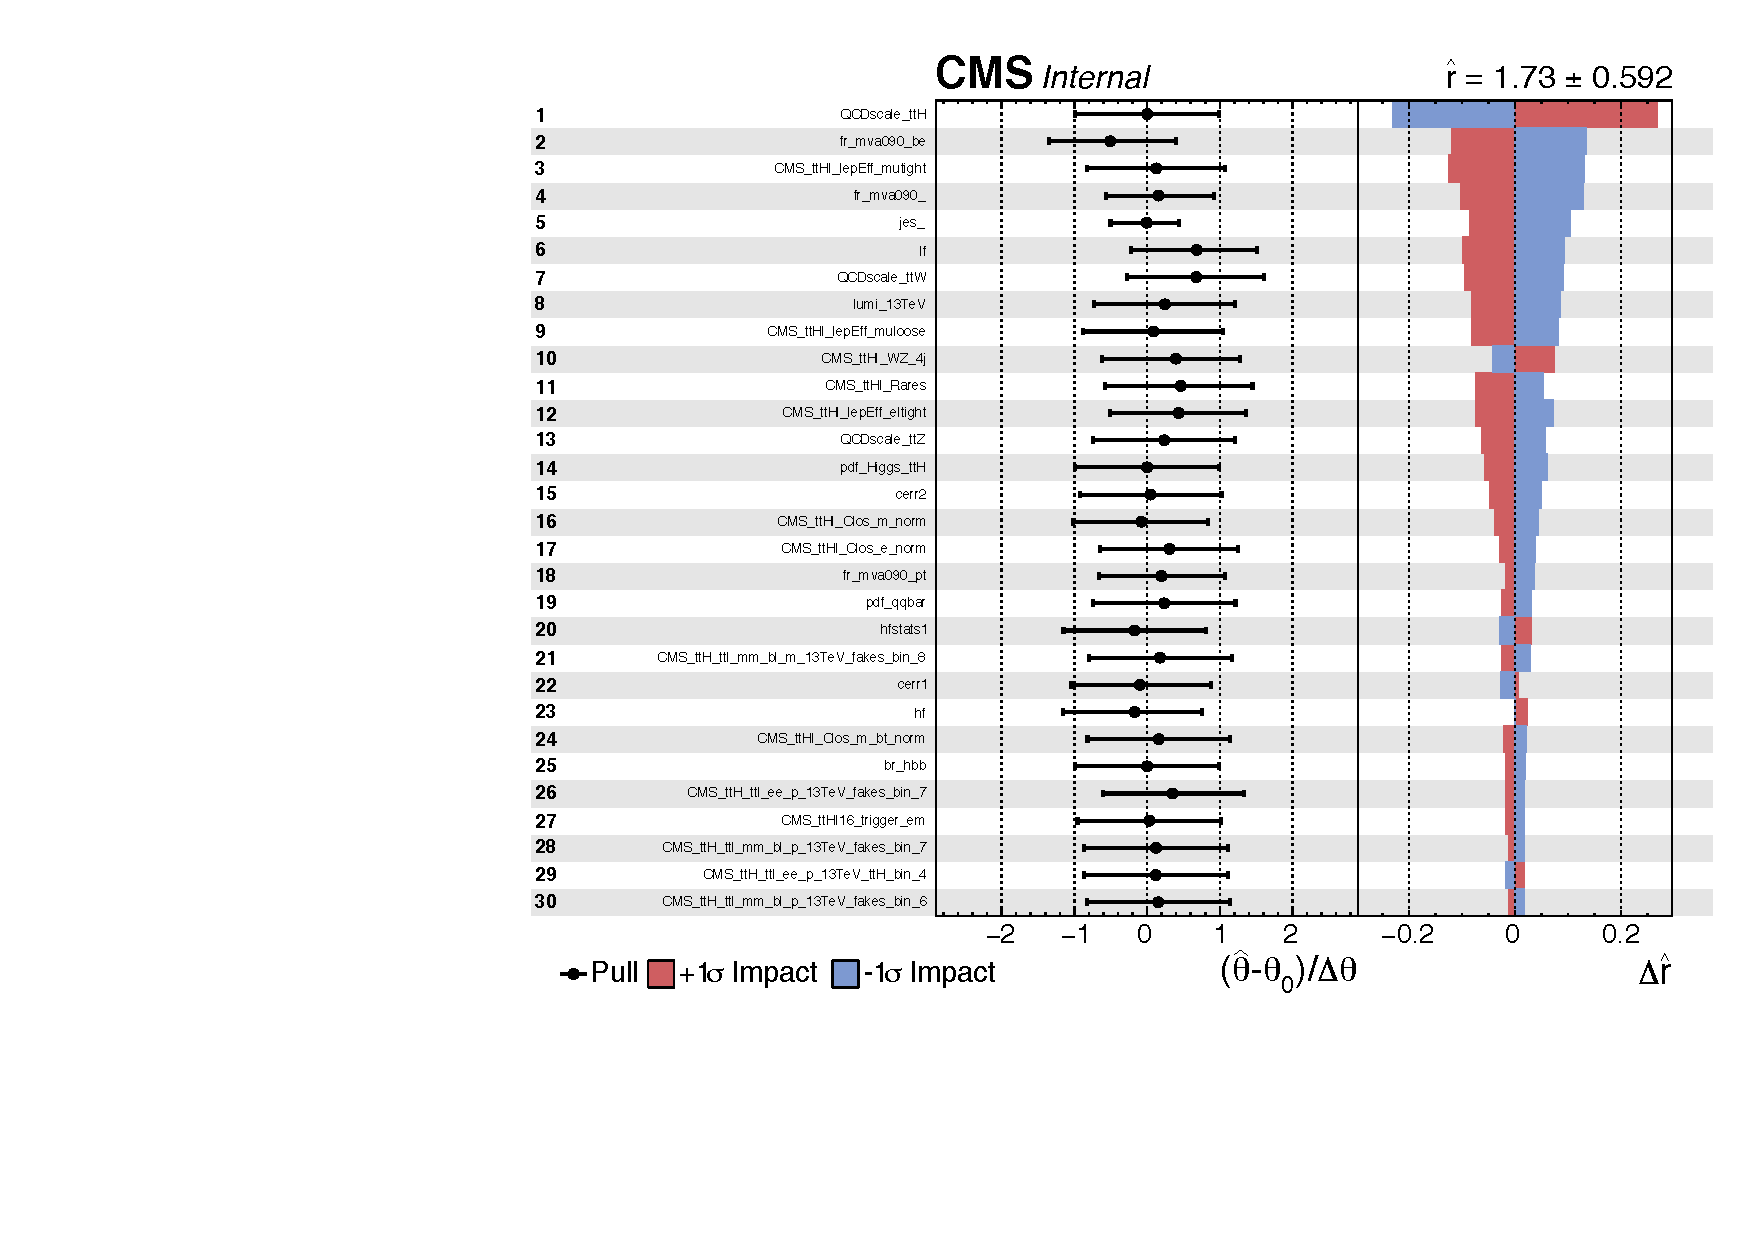
\includegraphics[width=0.95\textwidth]{ch10_figs/impacts_ttH_13TeV_top30.pdf}
        \caption[Nuisance parameter impacts]{The top nuisance parameters ranked by their impact on the fit. The relative pull of each nuisance (left) is the amount by which the fit moves each nuisance
          parameter from its initial value, divided by the post-fit uncertainty. The impact of each nuisance (right) is the change in best-fit $\mu$ divided by the uncertainty in $\mu$, obtained by
          moving each nuisance up (red) or down (blue) by 1$\sigma$ from the post-fit value. Note the change in notation for the POI: here $r$ is used to represent signal strength, normally represented with $\mu$.}
        \label{fig:impacts}
\end{figure}

\section{Upper Limits: CLs Method}
\label{sec:limit}
When an analysis lacks the sensitivity to discriminate signal from background, setting uppper limits on the possible values of $\mu$ is paramount. In setting upper
limits, $\mu$ is constrained as phase space of $\mu$ values is reduced and more values excluded. This strategy was used by the Higgs analyses at LEP and the Tevatron, and is the primary figure of merit
for an analysis with little sensitivity.
The \tth analysis presented here does not fall exclusively into this category as it has some sensitivity to \tth, although previous iterations lacked the sensitivity
to detect \tth in data. Upper limits are set using the CLs method, also known as the
Modified Frequentist approach, which builds on the likelihood described in the previous section. 

Starting from the likelihood in Equation~\ref{eqn:likelihood3}, we construct a test statistic, $q_{\mu}$, based on the profile likelihood ratio~\cite{AsymptoticLimits},
defined as:

\begin{equation}
\label{eqn:test_stat}
\tilde{q}_{\mu} = -ln \frac{\mathcal{L}(data|\mu,\hat{\theta}_{\mu})}{\mathcal{L}(data|\hat{\mu},\hat{\theta})},~~~~~~~~~0 \leq \hat{\mu} \leq{\mu}
\end{equation}

\noindent where $\hat{\theta}_{\mu}$ is the best-fit value of the nuisance parameters resulting from maximizing $\mathcal{L}(data|\mu,\hat{\theta}_{\mu})$ at a fixed $\mu$. 
The denominator, $\mathcal{L}(data|\hat{\mu},\hat{\theta})$, is the maximum likelihood obtained
previously where both parameters float. The lower bound $0 \leq \hat{\mu}$ ensures the signal is positive.
The upper bound $\hat{\mu} \leq \mu$ is imposed to produce a one-sided confidence interval. This also prevents upward fluctuations of data $\hat{\mu} > \mu$, 
from being considered as evidence against the signal hypothesis (a signal strength of $\mu$).

With the definition of the test statistic, we calculate $\tilde{q}_{\mu}^{obs}$, the observed test statistic value in data,
for many values of $\mu$, obtaining the values for the nuisance parameters observed in data, $\hat{\theta}_{0}^{obs}$, $\hat{\theta}_{\mu}^{obs}$
from maximizing the likelihoods under the background-only ($\mu=0$), and signal-plus-background hypotheses respectively.
Next, two test statistic PDFs
$f(\tilde{q}_{\mu}|\mu,\hat{\theta}_{\mu}^{obs})$, and $f(\tilde{q}_{\mu}|0,\hat{\theta}_{0}^{obs})$ are typically constructed from psuedo-data
generated with MC toys, obtained from random sampling of nuisance parameter values from the fit to data at fixed $\mu$, however this analysis uses an alternative
asymptotic approximation to generate these PDFs. Next we calculate a p-value $p_{\mu}$, $p_{b}$
for the signal-plus-background and background-only hypotheses. The p-value $p_{\mu}$ represents the probability that the observed data is incompatible with the
signal-plus-background hypothesis, with signal strength $\mu$.
The p-value $p_{b}$ is the probability for compatibility with the background-only hypothesis.
It is more convenient to work with $1-p_{b}$, since this value is the probability of incompatibility with the background-only hypothesis,
just as $p_{\mu}$ is a probability of incompatibility with the signal-plus-background hypothesis:

\begin{equation}
\label{eqn:pvalues1}
p_{\mu} = P(\tilde{q}_{\mu} \geq \tilde{q}_{\mu}^{obs}|signal+background) = \int_{\tilde{q}_{\mu}^{obs}}^{\infty} f(\tilde{q}_{\mu}|\mu,\hat{\theta}_{\mu}^{obs}) d\tilde{q}_{\mu}
\end{equation}

\begin{equation}
\label{eqn:pvalues2}
1- p_{b} = P(\tilde{q}_{\mu} \geq \tilde{q}_{\mu}^{obs}|background-only) = \int_{\tilde{q}_{0}^{obs}}^{\infty} f(\tilde{q}_{\mu}|0,\hat{\theta}_{0}^{obs}) d\tilde{q}_{\mu}
\end{equation}

\noindent We define confidence levels (CL) for each hypothesis, with $CL_{s+b} = p_{\mu}$, and $CL_{b} = 1-p_{b}$, with $CL_{s}$ being the ratio of the two:

\begin{equation}
\label{eqn:cls}
CL_{s}(\mu) = \frac{CL_{s+b}}{CL_{b}} = \frac{p_{\mu}}{1-p_{b}}
\end{equation}

\noindent Interpreting Equation~\ref{eqn:cls}, we can say that as the probability for incompatibility with the background-only hypothesis increases, and/or as the probability
for incompatibility with the signal-plus-background hypothesis decreases, $CL_{s}(\mu)$ will decrease, and we become more confident that the observed data is more consistent with
the signal-plus-background hypothesis than the background-only hypothesis. The observed 95$\%$ CL upper limit on $\mu$ is obtained by testing different values of decreasing $\mu$ and
calculating $CL_{s}(\mu)$, the upper limit is the value of $\mu$ for which $CL_{s}(\mu) = 0.05$. In general we say that for some $\mu$ corresponding to $CL_{s}(\mu) \leq \alpha$
greater values of $\mu$ are excluded at the $1-\alpha$ CL level. 

\begin{figure}[htb]
        \centering 
        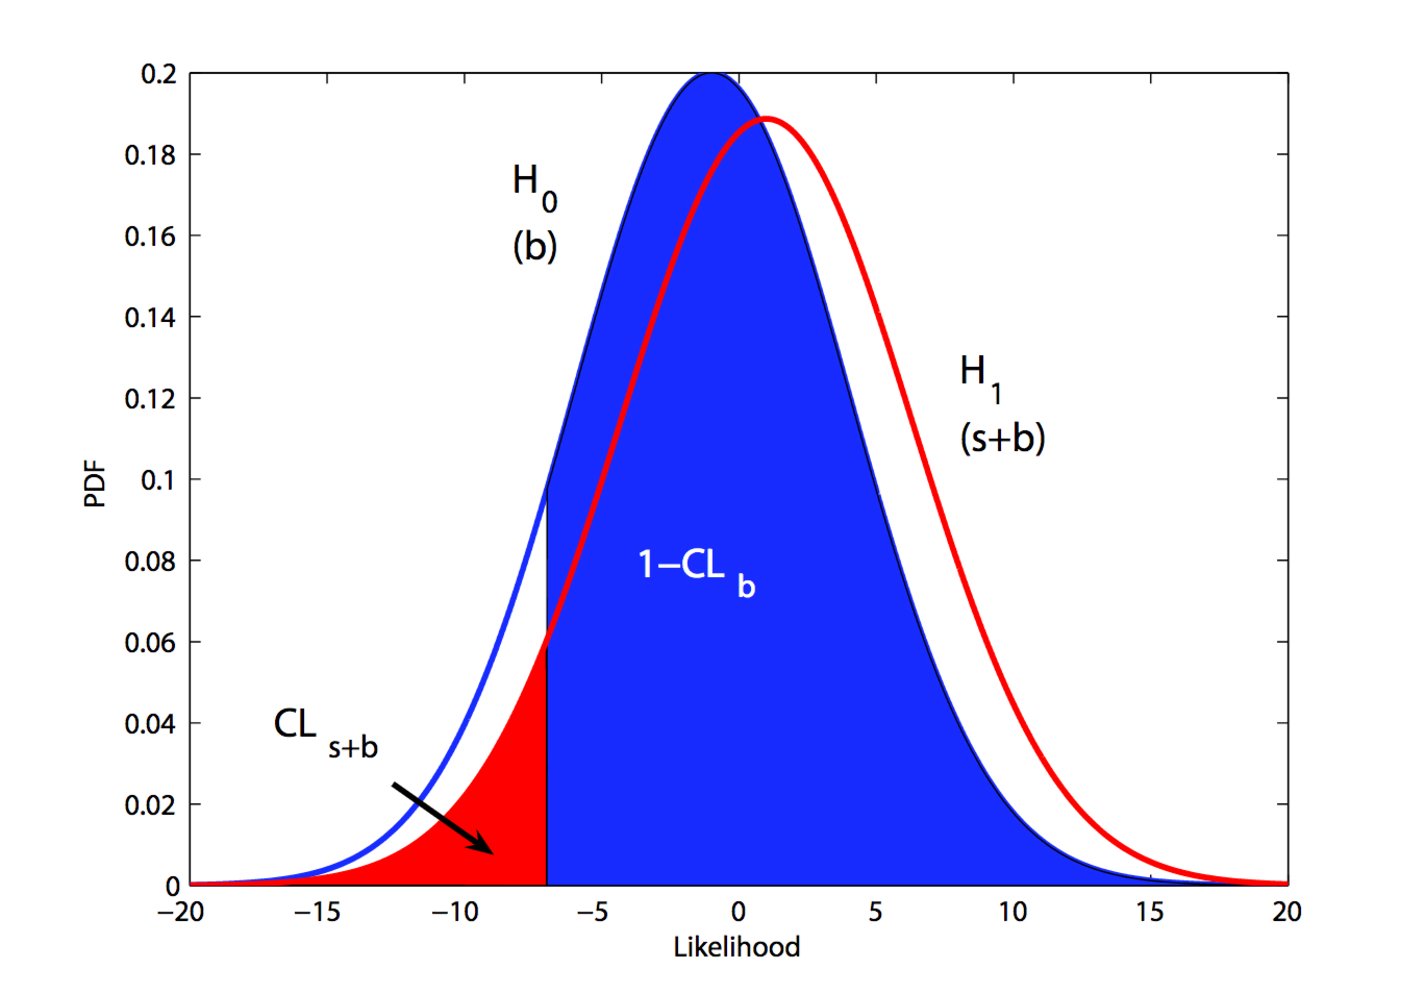
\includegraphics[width=0.80\textwidth]{ch10_figs/cls.pdf}
        \caption[Test statistic PDFs for s+b and b-only hypotheses]{An example of the signal-plus-background (red, $H_{1}$) and background-only (blue, $H_{0}$) PDFs for a
          test statistic (labeled 'likelihood' on the x-axis). The $(1-\alpha)\%$ CL upper limit is the value of $\mu$ which corresponds to x-axis value
          when $\frac{CL_{s+b}}{CL_{b}} \leq \alpha$~\cite{lhc4peds}.}
        \label{fig:cls}
\end{figure}

The expected upper limit is calculated by generating the background-only distribution from MC toys as described previously, for many pseudo experiments, calculating $CL_{s}$, $\mu^{95\% CL}$
for each distribution (pseudo experiment). Then a cumulative distribution of $\mu^{95\% CL}$ is constructed and the median expected value on the upper limit of $\mu$ is reported - which is the value
of $\mu^{95\% CL}$ for which the cumulative distribution crosses the 50$\%$ quantile\footnote{Technically, generating N toys for M pseudo experiments yields N$\cdot$M likelihood evaluations. Since the test-statistic
distributions for a given $\mu$ don't depend on the pseudo data, they are instead computed only once per $\mu$ value, and the total number of likelihood evaluations is proportional to N+M instead.}.

Generating large statistics of toy MC to produce the test statistic distributions needed for the method above is both time consuming and CPU intensive. This analysis uses an alternate method to
construct the test statistic distributions analytically, without the need for pseudo data, called the asymptotic approximation of the profile likelihood~\cite{AsymptoticLimits}.  
This procedure begins by removing the requirement that the signal be positive $\hat{\mu} > 0$ from the test statistic in Equation~\ref{eqn:test_stat}. From Wilks theorem
in the asymptotic regime, the test statistic will have half a $\chi^{2}$ distribution for one degree of freedom in the signal-plus-background hypothesis~\cite{wilks}. The value of $\mu$ for which
$\frac{1}{2}q_{\mu} = 1.92$ has the convenient property of corresponding to $CL_{s} = 0.05$. By imposing $\hat{\mu} > 0$, the asymptotic behavior of the test statistic PDF under the signal plus
background hypothesis no longer is half a $\chi^{2}$, but does follow a well-defined distribution:

\begin{equation}
\label{eqn:asymptote}
f(\tilde{q}_{\mu}|\mu) = \frac{1}{2}\delta(\tilde{q}_{\mu}) + \begin{cases}
  \frac{e^{-\tilde{q}_{\mu}/2}}{\sqrt{8\pi~\tilde{q}_{\mu}}} & ~~~~ 0 < \tilde{q}_{\mu} \leq \mu^{2}/\sigma^{2} \\
  \frac{e^{\frac{\tilde{q}_{\mu}+(\mu^{2}/\sigma^{2})}{8\mu^{2}/\sigma^{2}}}}{\sqrt{8\pi\mu^{2}/\sigma^{2}}} & ~~~~ \tilde{q}_{\mu} > \mu^{2}/\sigma^{2}
  \end{cases}
\end{equation}

\noindent where $\sigma^{2} = \mu^{2}/q_{\mu,A}$, and $q_{\mu,A}$ is known as the Asimov dataset\footnote{The Asimov dataset is named after the 1955 short story ``Franchise'' by Issac Asimov, where the 2008
U.S. election is determined by a single vote of one person, who is said to represent the entire population.} with all nuisances set to their initial values. The test statistic distributions for
signal-plus-background and background-only hypotheses are constructed from Equation~\ref{eqn:asymptote} instead of from toy MC~\cite{CMS-AN-11-298}. 

The 95$\%$ upper limits on $\mu$ are obtained with the $CL_{s}$ method using the asymptotic approximation of the profile likelihood, described in Section~\ref{sec:limit}.
The observed (median expected under background-only hypothesis) upper limit on $\mu$ is 2.9 (1.0$^{+0.5}_{-0.3}$), as shown in Table~\ref{tab:limits}.

\begin{table}[htbp]
\begin{center}
  \caption[Table of Final Limits]{95$\%$ CL upper limits on $\mu$ under the background-only hypothesis.}
    \begin{tabular}{c c} \hline
      Observed Limit & Expected Limit $\pm$1$\sigma$  \\ \hline 
      2.9 & 1.0$^{+0.5}_{-0.3}$  \\
      \hline
    \end{tabular}
    \label{tab:limits}
\end{center}
\end{table}



\section{Significance}
To determine the significance of the result, we use the asymptotic approximation of the profile likelihood described above. We calculate the probability of an observation that is compatible with the
data in the background-only hypothesis. This is the probability that the background randomly fluctuated to produce the observation in data. The lower this probability, the greater the significance.
This is expressed as a p-value, $p_{0}$:

\begin{equation}
\label{eqn:signif1}
p_{0} = P(q_{0} \geq q_{0}^{obs}) = \int_{q_{0}^{obs}}^{\infty} f(q_{0}|0,\hat{\theta_{0}^{obs}}) dq_{0}
\end{equation}

\noindent This p-value is converted into a significance, $Z$ (in units of standard deviations, $\sigma$) by integrating one side of the gaussian tail:

\begin{equation}
\label{eqn:signif2}
p_{0} = \int_{Z}^{\infty} \frac{1}{\sqrt{2\pi}}e^{-x^{2}/2} dx
\end{equation}

\noindent The value of $Z$ represents the number of standard deviations the background, assuming no signal, would have to fluctuate by to be consistent with the observation. 
The significance can also be approximated under the asymptotic profile likelihood with the test statistic defined in Equation~\ref{eqn:test_stat} under the background-only hypothesis:

\begin{equation}
\label{eqn:signif3}
Z = \sqrt{q_{0}}
\end{equation}

In high energy physics searches, a result with a significance of 3$\sigma$ or greater is considered  ``evidence'', while a result with 5$\sigma$ or greater significance
is considered an ``observation'' or ``discovery''. A significance of 3$\sigma$ corresponds to a p-value of 0.135$\%$, while a significance of 5$\sigma$ corresponds to a p-value
of 0.000029$\%$. The p-values represent the probability, under the background-only hypothesis, that the backgrounds randomly fluctuated to produce the observation.
